\section*{Problem 1}
	\begin{proof} [Solution]
		They are $G$ and $\overline{G}$.
		\begin{figure} [!htb]
			\subfloat[$G$]{{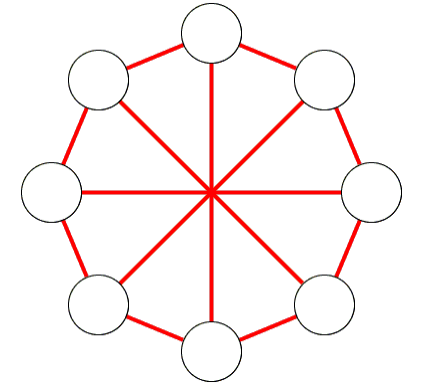
\includegraphics[width=0.47\textwidth]{G.png}}}
			\subfloat[$\overline{G}$]{{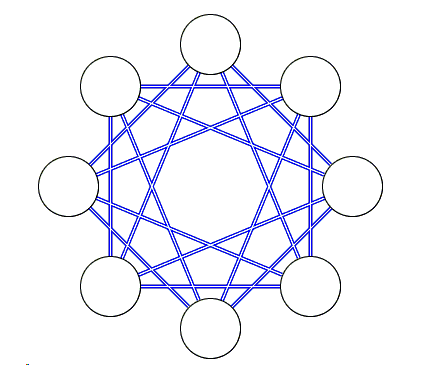
\includegraphics[width=0.5\textwidth]{G_.png}}}
		\end{figure}\\
		Since $G$ does not contain $K_3$ and $\overline{G}$ does not contain $K_4$, by the definition of \textit{Ramsey number}, it is a counter example for $R(3, 4) = 8$. Therefore, $R(3, 4) > 8$.\\
	\end{proof}